% \documentclass{easychair}
\documentclass[EPiC]{easychair}
%\documentclass[EPiCempty]{easychair}
%\documentclass[debug]{easychair}
%\documentclass[verbose]{easychair}
%\documentclass[notimes]{easychair}
%\documentclass[withtimes]{easychair}
%\documentclass[a4paper]{easychair}
%\documentclass[letterpaper]{easychair}

\usepackage{doc}
\usepackage{float}
\usepackage{amssymb}

\newenvironment{packed_itemize}{
\vspace*{-0.5em}
\begin{itemize}
  \setlength{\partopsep}{0pt}
  \setlength{\itemsep}{1pt}
  \setlength{\parskip}{0pt}
  \setlength{\parsep}{0pt}
}{\end{itemize}}

\newenvironment{packed_enumerate}{
\vspace*{-0.5em}
\begin{enumerate}
  \setlength{\partopsep}{0pt}
  \setlength{\itemsep}{1pt}
  \setlength{\parskip}{0pt}
  \setlength{\parsep}{0pt}
}{\end{enumerate}}

% use this if you have a long article and want to create an index
% \usepackage{makeidx}

% In order to save space or manage large tables or figures in a
% landcape-like text, you can use the rotating and pdflscape
% packages. Uncomment the desired from the below.
% \usepackage{rotating}
% \usepackage{pdflscape}

% Make sure to include the slash at the end of the path name
\graphicspath{ {./figures/} }

% Macros
\DeclareMathOperator*{\argmaxA}{arg\,max} % Jan Hlavacek - argmax function

%\makeindex

%% Front Matter
%%
% Regular title as in the article class.
%
\title{Evaluation of Axiom Selection Techniques}
% \thanks{Other people who contributed to this document include Maria Voronkov
%   (Imperial College and EasyChair) and Graham Gough (The University of
%   Manchester).}}

% Authors are joined by \and. Their affiliations are given by \inst, which indexes
% into the list defined using \institute
%
\author{
Qinghua Liu\inst{1}
 \and
Zishi Wu\inst{2}
 \and
Zihao Wang\inst{2}
 \and
Geoff Sutcliffe\inst{2}
% \thanks{Did numerous tests and provided a lot of suggestions}
}

% Institutes for affiliations are also joined by \and,
\institute{
  School of Information Science and Technology, Southwest Jiaotong University, China, \email{qhliu@my.swjtu.edu.cn}
\and
   University of Miami, USA, \email{zishi@cs.miami.edu,zxw526@miami.edu,geoff@cs.miami.edu}
 }

%  \authorrunning{} has to be set for the shorter version of the authors' names;
% otherwise a warning will be rendered in the running heads. When processed by
% EasyChair, this command is mandatory: a document without \authorrunning
% will be rejected by EasyChair

\authorrunning{Liu, Wang, Wu, Sutcliffe}

% \titlerunning{} has to be set to either the main title or its shorter
% version for the running heads. When processed by
% EasyChair, this command is mandatory: a document without \titlerunning
% will be rejected by EasyChair
\titlerunning{Evaluation of Axiom Selection Techniques}

\begin{document}

\maketitle
%------------------------------------------------------------------------------
\begin{abstract}
``Large Theory'' problems in Automated Theorem Proving have been
defined as having {\em many functors and predicates, and many axioms of
which only a few are required for the proof of a theorem}.
One key to solving large theory problems is selecting a subset of the axioms
that is adequate for finding a proof.
This paper presents metrics for evaluating axiom selection techniques
without having to run an ATP system on the problems formed from selected
axioms and the conjecture.
This paper additionally presents some new axiom selection techniques.
The new techniques, and the axiom selection in the Vampire ATP 
system, are evaluated using the proposed metrics.
\end{abstract}
%------------------------------------------------------------------------------
\section{Introduction}
\label{Introduction}

``Large Theory'' problems in Automated Theorem Proving (ATP) have been 
defined \cite{Sut20-CASC} as having {\em many functors and predicates, and 
many axioms of which only a few are required for the proof of a theorem}.
Large theory problems are mostly found in corpora that contain very many
problems, e.g., the MPTP2078 corpus \cite{AH+14}, the Mizar 40 corpus
\cite{KU15-M40}, and the GRUNGE corpus \cite{BG+19}.
Large theory problems present challenges to ATP systems, mainly because of the
large search space generated by the large number of axioms.
Thus one key to solving large theory problems is selecting a subset of the 
axioms that is adequate for finding a proof. 
There has been significant and successful research on this topic, e.g.,
\cite{PSZG04,SP07,MP09,KC+10,HV11,Kv+12,AH+14,GK15,PU18}.
Many techniques are based on the occurrences of symbols in the formulae,
e.g., the SInE method \cite{HV11} and its derivatives. 
The fact that large theory problems often occur in large corpora makes the
application of machine learning techniques \cite{KB14} viable, e.g., as 
done in the MaLARea system \cite{US+08}.

Evaluation of axiom selection techniques is typically done by:
\begin{packed_enumerate}
\item Choosing a corpus of large theory problems.
\item For each problem in the corpus, selecting a subset of the axioms.
\item Running an ATP system on a reduced problem formed from the selected 
      axioms and the problem's conjecture.
\end{packed_enumerate}
In the third step of this process, a proof indicates an adequate selection,
and a countermodel indicates an inadequate selection. 
However, time limits are imposed on ATP system runs, and when experiments 
are done on large corpora it is often necessary to impose a small time limit.
Time limits cause timeouts, and a timeout in the third step provides no 
information - the selection might be inadequate, or the selection might be 
adequate but the reduced problem is too hard because too many (unnecessary) 
axioms were selected or the time limit is too small.
The results are also influenced by the choice of ATP system.

This paper presents metrics for evaluating axiom selection techniques
without having to run an ATP system on the reduced problems.
While the ``proof is in the pudding'' and it is eventually necessary to
evaluate by running an ATP system, the method described in this paper
provides a first-pass evaluation that allows axiom selection techniques to
be rapidly tested and refined.
The approach has the advantage of being independent of a chosen ATP system.
This paper additionally presents some new axiom selection techniques. 
The new techniques and the axiom selection in the Vampire \cite{KV13} 
ATP system are evaluated using the proposed metrics.

This paper is structured as follows:
Section~\ref{Metrics} describes the evaluation metrics.
Section~\ref{Ours} describes a distance measure between formulae, and
some new axiom selection techniques based on that measure.
Section~\ref{Results} provides evaluation results.
Section~\ref{Conclusion} concludes.

%------------------------------------------------------------------------------
\section{Axiom Selection Metrics}
\label{Metrics}

The principle behind the new evaluation metrics is to compare a selected
subset of axioms with known adequate sets of axioms.
In this work the MPTP2078 corpus was used.
The MPTP2078 corpus has two versions of each of the 2078 problems: 
the \emph{bushy} (small) versions contain only the Mizar axioms that are
known to be directly used in the proof of the conjecture, and 
the \emph{chainy} versions contain all the axioms that precede the conjecture
in the Mizar library order.
The bushy problems have between 10 and 67 axioms, while the chainy versions
have between 10 and 4563 axioms.

In order to extract known adequate sets of axioms for each problem, Vampire
and E \cite{SCV19} were run on the problems with a 300s CPU limit.
This produced proofs for 1486 of the bushy problems (1474 by Vampire and 1263
by E) and 1345 of the chainy problems (1333 by Vampire and 815 by E).
For each problem solved, the axioms used in the proof were extracted as
a known adequate set of axioms, and new problems formed from that adequate
sets with the corresponding conjecture.
These new problems were dubbed the \emph{pruney} problems.
Additionally, in testing the new axiom selection techniques described in 
Section~\ref{Ours} some further different adequate sets were found, and 
further pruney problems created.
This resulted in pruney problems for a further 65 of the bushy problems and
24 of the chainy problems.
For some problems multiple adequate sets of axioms were found, resulting in
a total of 1829 pruney problems for the 1551 bushy problems, and a total of
3093 pruney problems for the 1369 chainy problems.
The pruney problems have been been used to augment the MPTP2078 corpus.
The pruney problems provide adequate known sets of axioms against which
selected sets of axioms can be compared.

The smallest fraction of axioms in an adequate set ranges from 0.01 to 1.0
for the bushy problems, and from 0.0002 to 0.36 for the chainy problems.
The average fractions are 0.29 and 0.01, respectively.
These fractions show that accurate axiom selection can significantly reduce the
number of axioms to be considered, which in turn normally significantly
reduces the search space of an ATP system.
As is expected, the numbers are more extreme for the larger chainy problems.

The metrics introduced in the paper aim to measure how precisely the
axiom selection matches a known adequate set of axioms.
Two types of axiom selection technique are considered:
\begin{itemize}
\item \emph{Ranking} techniques, which take all the axioms as input, rank them
      according to how likely they are to be necessary for a proof,
      and take the best ones from the ranking.
      This technique is used in, e.g., Isabelle's Sledgehammer \cite{PB10}.
\item \emph{Projection} techniques, which take all the axioms as input and
      directly return a selection of axioms.
      (Ranking is thus a special case of projection.)
      This technique is used in, e.g., Vampire \cite{HV11}.
\end{itemize}

Define the following measures:
\begin{packed_itemize}
\item The \emph{n}umber of \emph{ax}ioms in a \emph{p}roblem: \emph{NAxP}.
\item The \emph{n}umber of axioms \emph{sel}ected: \emph{NSel}.
\item The \emph{n}umber of axioms \emph{n}eeded \emph{f}or a \emph{p}roof, 
      i.e., the number of axioms in an adequate set: \emph{NNfP}.
\item In a ranked list of axioms, the number of axioms down to the lowest ranked
      axiom needed for a proof, i.e., the \emph{n}umber of axioms
      \emph{n}eeded from the \emph{ra}nking: \emph{NNRa}.
\end{packed_itemize}

The axiom selection metrics are:

\paragraph{Precision.}
If the selection technique selects an adequate set of axioms, i.e., a subset
of one of the known adequate sets, then the minimum \emph{NNfP}$/$\emph{NSel},
over the known adequate sets.
If the selection technique selects an inadequate set, then $0.00$.
Larger values are better.
The intuition here is a probability that using the selection will result
in a proof (and that is $0.00$ if an inadequate set is selected).

\paragraph{Selectivity.}
\emph{NSel}$/$\emph{NAxP}.
This measures the fraction of axioms selected.
$1.00$ results from selecting all the axioms - the base case.
Smaller values are better.

\paragraph{Ranking precision.}
(Applicable to only ranking techniques.)
If the selection technique selects an adequate set of axioms, then
\emph{NNRa}$/$\emph{NSel}.
If the selection technique selects an inadequate set, then $0.00$.
This measures how precisely the technique chooses the ``best ones'' from
the ranked list of axioms.
Larger values are better.

\paragraph{Ranking density.}
(Applicable to only ranking techniques.)
\emph{NNfP}$/$\emph{NNRa}.
This measures the quality of the ranking - axioms in an adequate set should
be ranked highly, which in turn allows a smaller number to be selected if
the ranking precision is good.
Larger values are better.

\paragraph{Average precision/selectivity/ranking precision/ranking density.}
For a set of problems, the average over the problems.

\paragraph{Adequacy.}
For a set of problems, the adequacy is the fraction of problems for which
the selection technique selects an adequate set of axioms.
Larger values are better.

\paragraph{Adequate precision/selectivity/ranking precision/ranking density.}
For a set of problems, the average over the problems for which the selection 
technique selects an adequate set of axioms.

%------------------------------------------------------------------------------
\section{Our Selection Techniques}
\label{Ours}

Our motivation for developing these metric was based in a need to evaluate
new axiom selection techniques that the first three authors were developing.
These techniques are described in this section, and their performance
according to the metrics is evaluated in Section~\ref{Results}.
It turns out that a very simply technique performs surprisingly well
on the MPTP2078 corpus.

All of the new techniques are based on how strongly two formulae are
related (as is the case in many axiom selection techniques).
In our work we use a novel measure of relatedness, which is described
in Section~\ref{QinghuaDistance}.
The individual new techniques are then described in 
Sections~\ref{QinghuaInf}~to~\ref{Zihao}.

%------------------------------------------------------------------------------
\subsection{Formula Dissimilarity and Similarity}
\label{QinghuaDistance}

The relatedness between two formulae is computed first as a
\emph{dissimilarity} between the two formulae, which is also later converted
to a \emph{similarity}.
The dissimilarity between two atoms is an extended version of the
Hutchinson distance \cite{Hut97}.

For two terms or atoms $\Delta_1$ and $\Delta_2$, their \emph{least general 
generalization} $\Delta = lgg(\Delta_1,\Delta_2)$, if it exists, is a term 
or atom $\Delta$ such that there are substitutions $\theta_1$ and $\theta_2$, 
$\Delta\theta_1 = \Delta_1$ and $\Delta\theta_2 = \Delta_2$, and 
there is no term or atom $\Delta'$ and substitutions 
$\sigma, \sigma_1, \sigma_2$ such that 
$\Delta\sigma = \Delta'$, $\Delta'\sigma_1 = \Delta_1$, 
and $\Delta'\sigma_2 = \Delta_2$.
If $lgg(\Delta_1,\Delta_2)$ does not exist, e.g., neither are variables and 
the principle symbols of $\Delta$ and $\Delta$ are different, then their 
dissimilarity $dsim(\Delta_1,\Delta_2) = \infty$.
Otherwise:

Divide $\theta_i$ into two parts, $\theta_i^v$ and $\theta_i^f$:
\begin{center}
$\theta_i^v=\{X_{i,1}\mapsto Z_{i,1},\dots,X_{i,m_i}\mapsto Z_{i,m_i}\}$
~~~~
$\theta_i^f=\{Y_{i,1}\mapsto f_{i,1},\dots,Y_{i,n_i}\mapsto f_{i,n_i}\}$
\end{center}
where $X_{i,j}$ and $Y_{i,j}$ are the substituted variables, 
$Z_{i,j}$ are substituting variables, and
$f_{i,j}$ are substituting functional terms.
Let
\begin{packed_itemize}
\item $w_v$ be a weight for variables (currently set to $1$).
\item $w_f$ be a weight function for non-variable symbols (currently
      set to $2$ for all symbols). 
\item $V(X,\Phi)$ be the set of occurrences of the variable $X$ in $\Phi$.
\item $N(X,\Phi)$ be the nesting level of the variable $X$ in $\Phi$, e.g., 
      $N(X,p(f(X)) = 2$.
\item $W_v(X,\Phi)$ be 
      $w_v \times (|V(X,\Phi)| + \sum_{U \in V(X,\Phi)} N(U,\Phi))$,
      i.e., the weighted sum of the number of occurrences of $X$ in $\Phi$ and 
      the nesting levels of the occurrences of $X$ in $\Phi$, e.g., 
      $W_v(X,p(X,f(X)) = w_v \times (2 + (1+2)) = 5$.
\item $W_f(\Phi)$ be the sum of the weights of all the non-variable symbols 
      occuring in $\Phi$.
\item $g(x)$ be a continuous increasing function 
      $\mathbb{R} \mapsto \mathbb{R}$ such that 
      $g(0)=0$
      % $g(x)\geq0$ for $x \geq 0$, 
      and
      $g(x_1+x_2) \leq g(x_1)+ g(x_2)$ for $x_1, x_2\geq0$
      (currently set to $ln(x+1)$).
% \item $occ(t,\Phi)$ denote the number of occurrences of $t$ in $\Phi$.
%\item $occ_{t}^{+}(v)$ denotes the number of deep occurrences of a variable 
%      $v$ in a term $t$, which takes the depth of $v$ (the number of symbols 
%      nested $v$) into consideration. 
%      For every occurrence $i$ of $v$, the depth of $v$ is $n_i$ ($n_i\geq$ 0). 
%      $occ_{t}^{+}(v)=\sum_{i=1}^{occ_{t}(v)}n_i+occ_{t}(v)$.
\end{packed_itemize}

Then, $S_f$ and $S_v$ are functions that map $\theta_i^v$ and 
$\theta_i^f$ to real numbers:
\begin{align}
S_v(\theta_i^v) &= \sum_{j=1}^{m_i} g(W_v(Z_{i,j},\Delta_i) - W_v(X_{i.j},\Delta)) \\
S_f(\theta_i^f) &= \sum_{j=1}^{n_i} (V(Y_{i,j},\Delta) \times W_f(f_{i,j}))
\end{align}
$S_v(\theta)$ measures the difference between the usage of substituting 
variables in $\Delta_i$ and the usage of substituted variables 
in $\Delta$, over the subsitutions made in $\Delta$ by $\theta_i^v$.
$S_f(\theta)$ measures the total function symbol weight of the substituting 
terms, over the substitutions made in $\Delta$ by $\theta_i^f$.

The dissimilarity between two atoms (or terms, but that is not of direct
interest in this work) $\Delta_1$ and $\Delta_2$ is then:
\begin{align}
dsim(\Delta_1,\Delta_2) = \sqrt{[S_v(\theta_1^v)+S_v(\theta_2^v)]^2+[S_f(\theta_1^f)+S_f(\theta_2^f)]^2}
\end{align}
The dissimilarity between two atoms measures the combined substitution
``effort'' required to convert their least general generalization to those 
atoms.

Let $\Phi_1$ and $\Phi_2$ be two formulae, containing the atoms
$\{\Delta_{1,1},\dots,\Delta_{1,n}\}$ and 
$\{\Delta_{2,1},\dots,\Delta_{2,m}\}$ respectively.
Let $S_{\neq\infty}$ be the set of pairs $(\Delta_{1,i},\Delta_{2,j})$ 
for which $dsim(\Delta_{1,i},\Delta_{2,j}) \neq \infty$.
If $S_{\neq\infty} = \emptyset$, i.e., all pairs of atoms are infinitely 
dissimilar, then the dissimilarity between $\Phi_1$ and $\Phi_2$ is 
$dsim(\Phi_1,\Phi_2) = \infty$.
Otherwise:
\begin{align}
dsim(\Phi_1,\Phi_2) = 
\frac{\sum_{(\Delta_{1,i},\Delta_{2,j}) \in S_{\neq\infty}}dsim(\Delta_{1,i},\Delta_{2,j})}
{|S_{\neq\infty}|}
\times
\frac{n \times m}{|S_{\neq\infty}|} 
\end{align}
The first term is the average dissimilarity between pairs of atoms that are 
not infinitely dissimilar.
The second term penalizes the first by the excess of atom pairs whose
dissimilarity is infinite.
Intuitively, the dissimilarity between two formulae measures the extent 
to which inference between them might not be possible by virtue of the 
dissimilarity of their atoms.

For two formulae $\Phi_1$ and $\Phi_2$, their similarity $sim(\Phi_1,\Phi_2)$
is defined in the context of a set of formulae $\mathcal{F}$, 
$\Phi_1,\Phi_2 \in \mathcal{F}$:
\begin{align}
maxdsim(\mathcal{F}) &= max_{\phi_i,\phi_j \in \mathcal{F}} (dsim(\phi_i,\phi_j) \neq \infty) \\
sim(\Phi_1,\Phi_2,\mathcal{F}) &= \textrm{max}(0, maxdsim(\mathcal{F}) - dsim(\Phi_1,\Phi_2))
\end{align}
If the dissimilarity is $0$, then the similarity is the largest dissimilarity 
that is not $\infty$.
If the dissimilarity is greater than $0$ and not $\infty$, then the similarity 
is the difference between the largest dissimilarity that is not $\infty$ and 
the dissimilarity.
If the dissimilarity is $\infty$ or is equal to the largest 
dissimilarity that is not $\infty$, then the similarity is $0$.

%------------------------------------------------------------------------------
\subsection{Q$\infty$}
\label{QinghuaInf}

This axiom selection technique takes a problem consisting of a conjecture 
$\mathcal{C}$ and axioms $\mathcal{A}$, and selects all axioms 
$\Phi \in \mathcal{A}$ such that $dsim(\mathcal{C},\Phi) \neq \infty$.
This simply means that each axiom contains at least one atom whose predicate
symbol matches that of an atom in the conjecture.

%------------------------------------------------------------------------------
% \subsection{A(nother) Machine Learning Approach}
% \label{QinghuaML}
% 
% 3. Qinghua's ML?
%------------------------------------------------------------------------------
\subsection{Spectral Clustering}
\label{Zishi}

This axiom selection technique views the formulae of a problem as nodes
of a complete graph, with the similarities between the formulae being the 
edge weights.
Spectral clustering \cite{vLu07} is then used to cluster together similar 
nodes, and the axioms in the cluster containing the conjecture are selected.
This process requires three steps:
determining the number of clusters,
choosing the initial centroids for the clusters,
and
applying k-means clustering.

The initial centriods for the clustering were extracted from a feature matrix 
consisting of the eigenvectors of the $L_{sym}$ normalized graph Laplacian 
matrix \cite{vLu07}, computed from the graph's adjacency matrix.
The rows of the feature matrix corresponding to the conjecture node and to 
the axiom nodes with highest degree centrality were used as the initial 
centroids.

To determine the number of clusters for a problem in the MPTP2078 corpus,
the three step process was applied to each problem with the number of 
clusters ranging from two to half the number of formulae in the problem.
The precision was computed each time, and the best number of clusters
recorded.
A median regression line was fitted to this data (separately for the
bushy and chainy problems), as shown in Figure~\ref{fig:median-regression}.
The regression lines were then used to set the number of clusters for
the final evaluation, based on the number of formulae in each problem.

\begin{figure}[h]
\centering
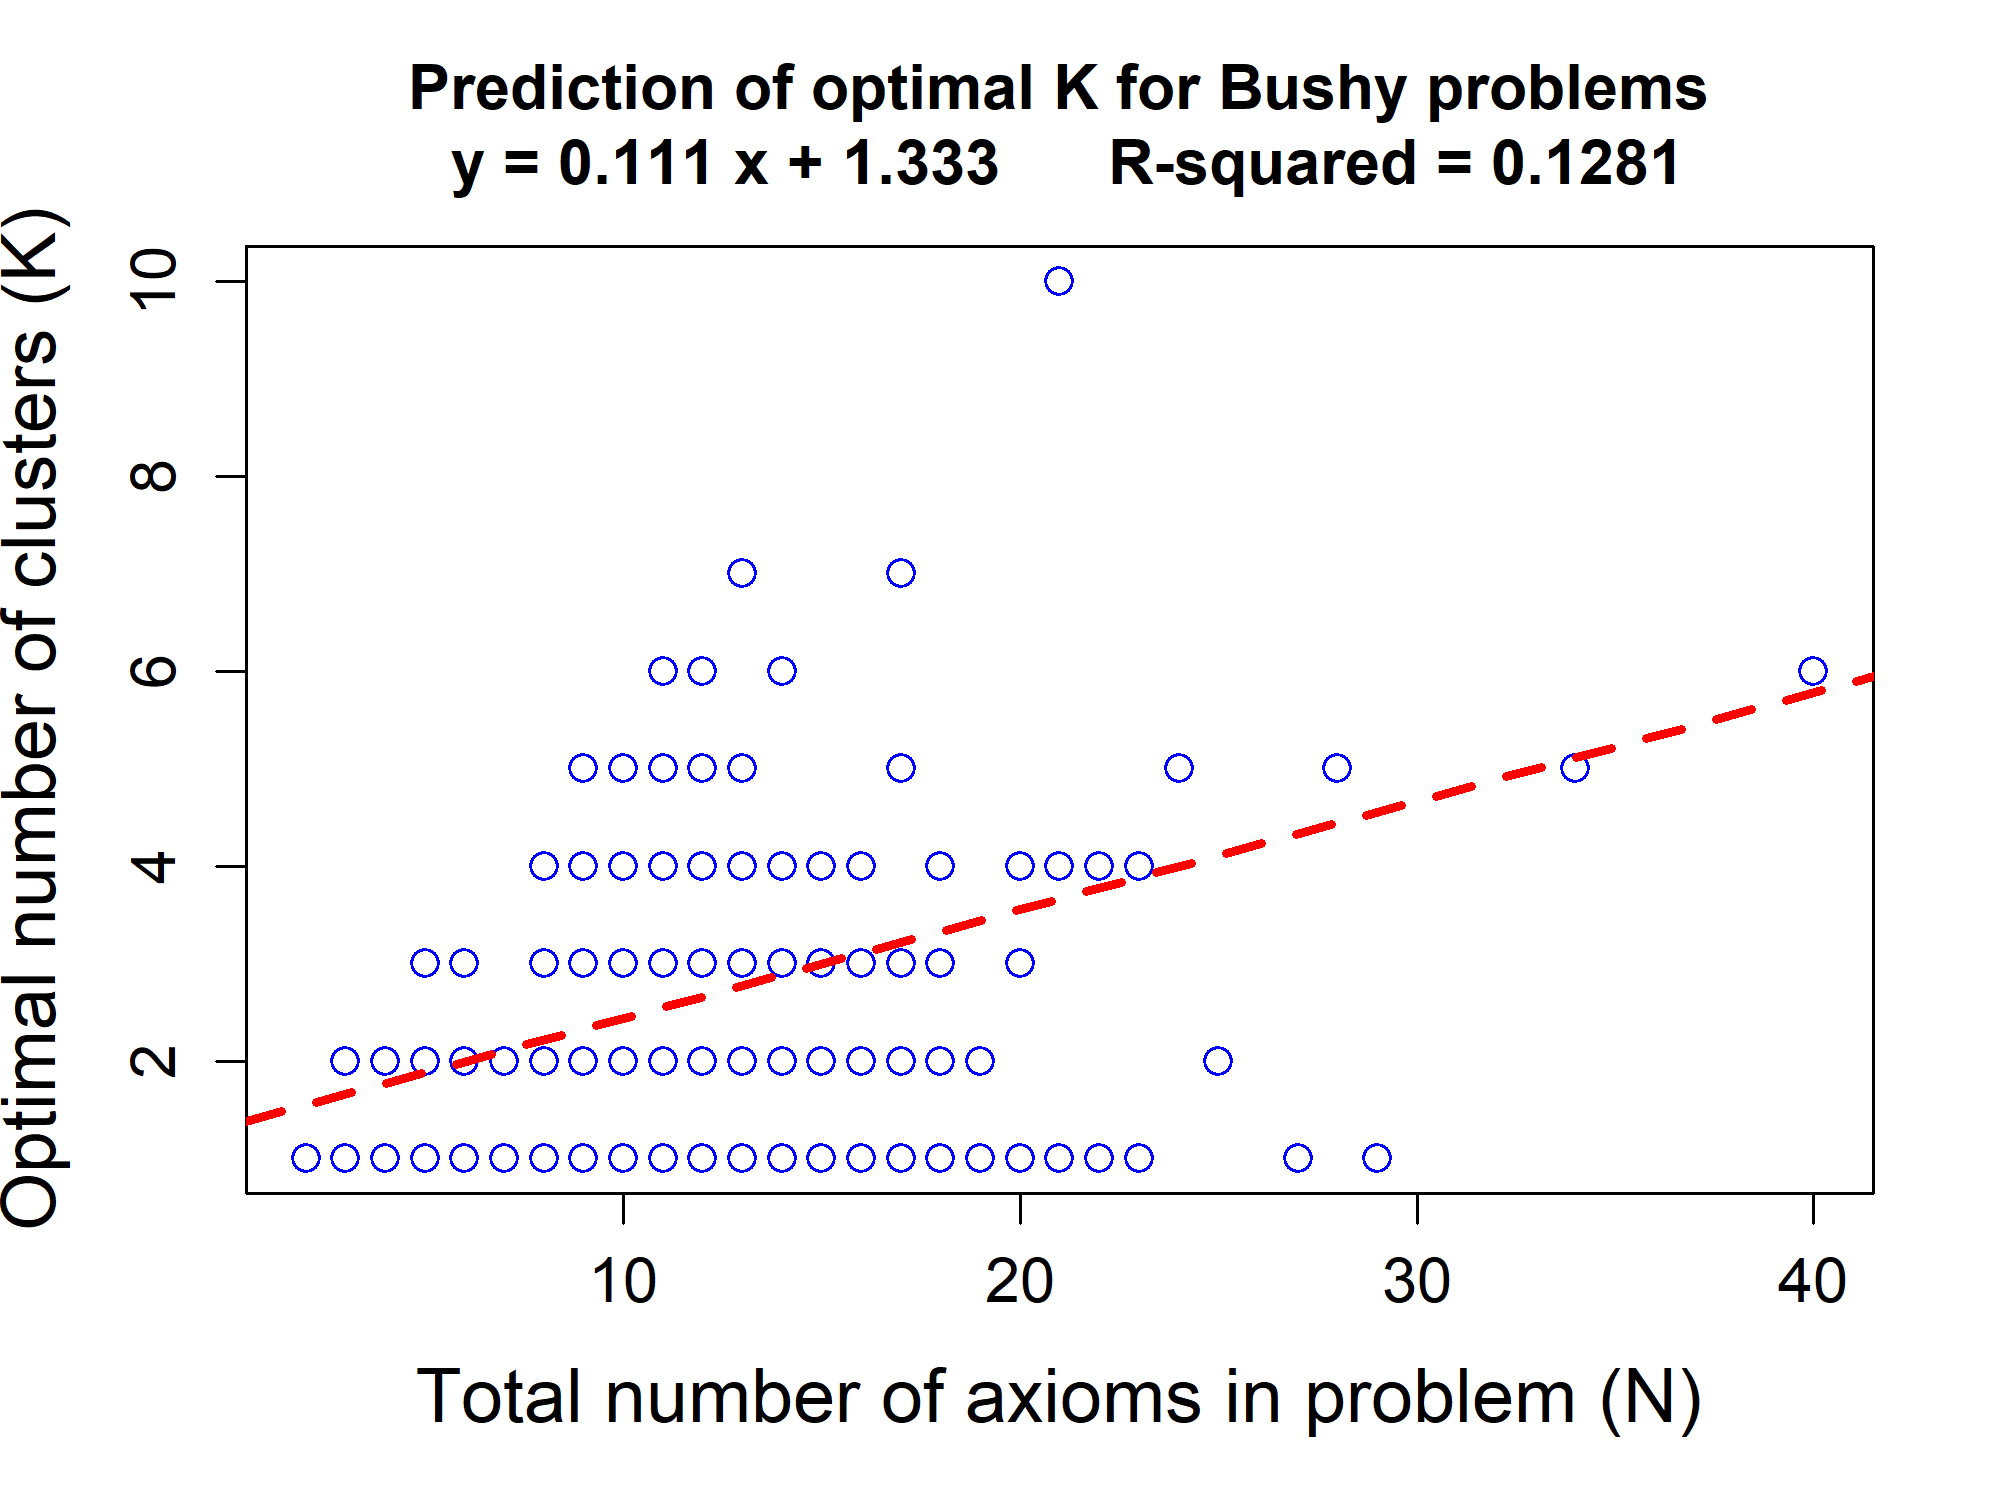
\includegraphics[scale=0.42]{median-regression-optimal-k-bushy.png}
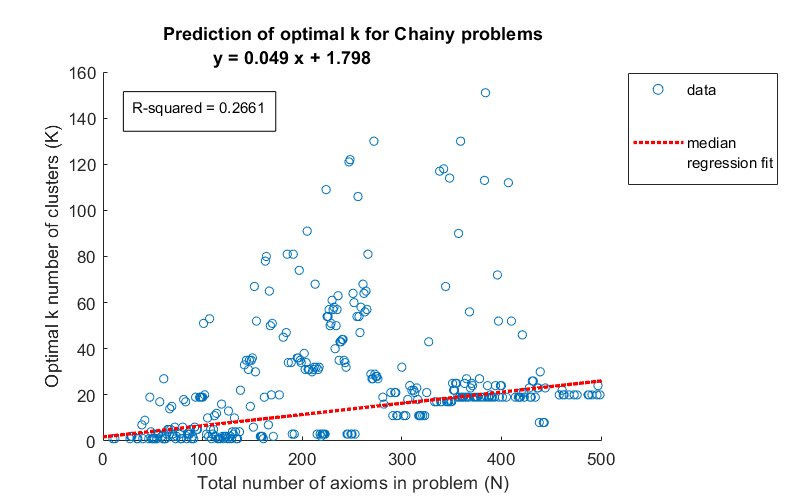
\includegraphics[scale=0.42]{median-regression-optimal-k-chainy.png}
\caption{Best number of clusters vs. Number of formulae}
\label{fig:median-regression}
\end{figure}

%------------------------------------------------------------------------------
\subsection{Greedy Tree +NN}
\label{Zihao}

As with the spectral clustering technique, this technique views the formulae
and their similarities as a complete graph.
Figure~\ref{GreedyTree} provides a simple illustrative example, in which
the {\sf C} node is the conjecture and the {\sf A} nodes are the axioms.
The edge weights are the similarities between the formulae (the figure
omits edges that do not affect the example).
Starting at the conjecture node, a greedy tree is built by iteratively 
visiting the nodes most similar to the current leaves of the tree, until 
nodes that have zero similarity (or equivalently, infinite dissimilarity) 
to the conjecture are reached, (these infinitely dissimilar nodes are 
ignored).
In Figure~\ref{GreedyTree} the thicker edges are those that are followed,
and the nodes with thicker circles are the nodes at which the tree growth 
stops because they that have zero similarity to the conjecture.
At that stage the light grey axiom nodes are in the tree.
As a final step, all the unvisited nodes most similar to the nodes in the 
greedy tree are added to the tree.
In Figure~\ref{GreedyTree}, that adds the dark grey axiom nodes to the 
tree.
The axiom nodes in the tree are selected.

\begin{figure}[h]
\centering
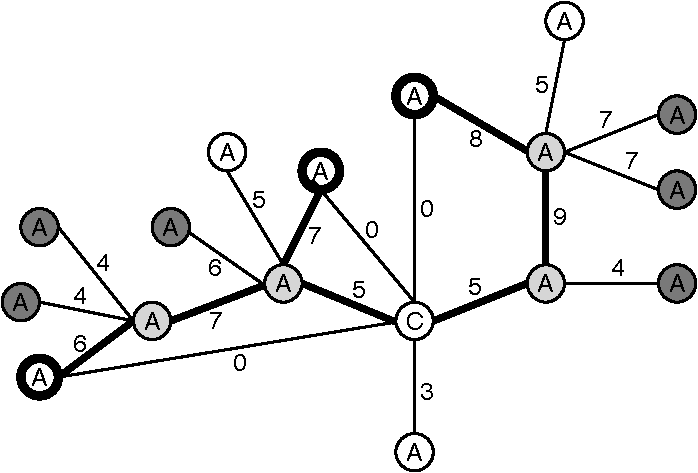
\includegraphics[width=0.5\linewidth]{GreedyTree+NN.pdf}
\caption{A greedy tree}
\label{GreedyTree}
\end{figure}

%------------------------------------------------------------------------------
\section{Evaluation Results}
\label{Results}

The new axiom selection techniques and the axiom selection in the Vampire 
ATP system were evaluated using the metrics.
Two problems sets from each of the bushy and chainy parts of the MPTP2078 
corpus were used. 
The first set was selected by taking the 325 chainy problems with less than 
500 axioms and for which adequate axiom sets (pruney problems) are known, 
and taking the corresponding 325 bushy problems.
The second set was the 1551 bushy problems and 1369 chainy problems for which
adequate axiom sets (pruney problems) are known.
The smaller set was useful for initial quick testing, and also necessary 
because some of the new techniques could not analyse the full set with the 
available computing resources.

Tables~\ref{Results325} and ~\ref{Results2078} show the results, including
a row for the base case in which all axioms are selected.
The columns are the 
Precision (Prcn), 
Selectivity (Sely), 
Ranking precision (RPrn), 
Ranking density (RDen), 
Adequacy (Adeq),
and the Adequate precision/selectivity/ranking precision/ranking density.

\begin{table}[hbt]
\begin{center}
\begin{tabular}{|l|rrrr|r|rrrr|}
\hline
325 Bushy problems  & \multicolumn{4}{|c|}{Average} & \multicolumn{5}{|c|}{Adequate} \\
Technique       & Prcn & Sely & RPrn & RDen & Adeq & Prcn & Sely & RPrn & RDen \\
\hline
Base            & 0.35 & 1.00 &  -   &  -   & 1.00 & 0.35 & 1.00 &  -   &  -   \\
% E 2.4           & 0.35 & 1.00 &  -   &  -   & 1.00 & 0.35 & 1.00 &  -   &  -   \\
Vampire 4.4     & 0.32 & 0.80 &  -   &  -   & 0.80 & 0.39 & 0.84 &  -   &  -   \\
Q$\infty$       & 0.43 & 0.54 & 0.62 & 0.52 & 0.74 & 0.58 & 0.61 & 0.84 & 0.71 \\
Spectral Cl.    & 0.24 & 0.57 &  -   &  -   & 0.66 & 0.36 & 0.79 &  -   &  -   \\
Greedy tree +NN & 0.37 & 0.77 &  -   &  -   & 0.97 & 0.38 & 0.80 &  -   &  -   \\
\hline
325 Chainy problems & \multicolumn{4}{|c|}{Average} & \multicolumn{5}{|c|}{Adequate} \\
Technique       & Prcn & Sely & RPrn & RDen & Adeq & Prcn & Sely & RPrn & RDen \\
\hline
Base            & 0.06 & 1.00 &  -   &  -   & 1.00 & 0.06 & 1.00 &  -   &  -   \\
% E 2.4           & 0.06 & 1.00 &  -   &  -   & 1.00 & 0.06 & 1.00 &  -   &  -   \\
Vampire 4.4     & 0.08 & 0.55 &  -   &  -   & 0.94 & 0.09 & 0.56 &  -   &  -   \\
Q$\infty$       & 0.08 & 0.53 & 0.57 & 0.21 & 0.85 & 0.09 & 0.56 & 0.67 & 0.25 \\
Spectral Cl.    & 0.05 & 0.48 &  -   &  -   & 0.65 & 0.08 & 0.63 &  -   &  -   \\
Greedy tree +NN & 0.05 & 0.93 &  -   &  -   & 0.96 & 0.05 & 0.96 &  -   &  -   \\
\hline
\end{tabular}
\caption{Results for the 325 smaller problems}
\label{Results325}
\end{center}
\end{table}

\begin{table}[hbt]
\begin{center}
\begin{tabular}{|l|rrrr|r|rrrr|}
\hline
1551 Bushy problems  & \multicolumn{4}{|c|}{Average} & \multicolumn{5}{|c|}{Adequate} \\
Technique       & Prcn & Sely & RPrn & RDen & Adeq & Prcn & Sely & RPrn & RDen \\
\hline
Base            & 0.30 & 1.00 &  -   &  -   & 1.00 & 0.30 & 1.00 &  -   &  -   \\
% E 2.4           & 0.30 & 1.00 &  -   &  -   & 1.00 & 0.30 & 1.00 &  -   &  -   \\
Vampire 4.4     & 0.21 & 0.69 &  -   &  -   & 0.58 & 0.36 & 0.76 &  -   &  -   \\
Q$\infty$       & 0.33 & 0.54 & 0.55 & 0.42 & 0.69 & 0.48 & 0.59 & 0.81 & 0.61 \\
\hline
1369 Chainy problems & \multicolumn{4}{|c|}{Average} & \multicolumn{5}{|c|}{Adequate} \\
Technique       & Prcn & Sely & RPrn & RDen & Adeq & Prcn & Sely & RPrn & RDen \\
\hline
Base            & 0.02 & 1.00 &  -   &  -   & 1.00 & 0.02 & 1.00 &  -   &  -   \\
% E 2.4           & 0.02 & 0.98 &  -   &  -   & 1.00 & 0.02 & 0.98 &  -   &  -   \\
Vampire 4.4     & 0.03 & 0.40 &  -   &  -   & 0.87 & 0.04 & 0.41 &  -   &  -   \\
Q$\infty$       & 0.03 & 0.53 & 0.46 & 0.07 & 0.83 & 0.04 & 0.56 & 0.56 & 0.08 \\
\hline
\end{tabular}
\caption{Results for all problems with known adquate axiom sets}
\label{Results2078}
\end{center}
\end{table}

For the smaller set of 325 bushy problems Q$\infty$ performs the best, with
the highest precision and lowest selectivity.
It also has a 74\% adequacy.
Moving up to the 325 chainy problems Q$\infty$ and Vampire have the highest
precision, with Q$\infty$ having slightly higher selectivity, and Vampire
better adequacy.
For the 1551 bushy problems Q$\infty$ is again the top performer, here in
terms of precision, selectivity, and adequacy.
Fnally, for the 1369 chainy problems Q$\infty$ and Vampire again have the 
highest precision, with Vampire having the best selectivity and adequacy.
The raw precision values are dissappointingly low, especially for the
chainy problems.
For Q$\infty$ the ranking density is similarly low, so that even with perfect
ranking precision the raw precision cannot be very good.
The adequacy numbers have to be viewed carefully - it is easy to get an
optimal adequacy, simply by selecting all axioms and thus having pessimal
selectivity.

As was noted in the introduction to this paper, while metrics such as
those presented in this paper are useful for quick evaluation of axiom
selection techniques, the ``proof is in the pudding''.
The quality of the metrics needs to be established by comparing them with 
eventual ATP system performance.
An intial evaluation of the precision metric has been performed by using
the Q$\infty$ axiom selection to produce reduced problems for the E ATP
system, and looking at the performance of E on the resultant reduced problems.
This was done for the 1551 bushy problems and 1369 chainy problems for
which there are known adequate axiom sets, so that the precision could
be computed.
The results are shown in Table~\ref{EvaluationOfMetrics}.

\begin{table}[hbt]
\begin{center}
\begin{tabular}{|l|rr|rr|rr|rr|}
\hline
                & \multicolumn{4}{|c|}{1551 Bushy problems} & \multicolumn{4}{|c|}{1369 Chainy problems} \\
                & \multicolumn{2}{|c|}{Unsolved} & \multicolumn{2}{|c|}{Solved} & \multicolumn{2}{|c|}{Unsolved} & \multicolumn{2}{|c|}{Solved} \\
\hline
\# Problems     &  604 & (39\%) &  947 & (61\%) &  681 & (50\%) &  691 & (51\%) \\
Avg Prcn        & 0.08 &        & 0.49 &        & 0.01 &        & 0.05 &        \\
\# Prcn 0       &  488 & (81\%) &    0 & (~0\%) &  232 & (34\%) &    0 & (~0\%) \\
\# Prcn 1       &    2 & (~0\%) &   63 & (~7\%) &    0 & (~0\%) &    0 & (~0\%) \\
\hline
\end{tabular}
\caption{Evaluation of Q$\infty$ wrt E}
\label{EvaluationOfMetrics}
\end{center}
\end{table}

%------------------------------------------------------------------------------
\section{Conclusion}
\label{Conclusion}

This paper has presented metrics for evaluating axiom selection techniques
without having to run an ATP system on the resultant reduced problems.
Some new axiom selection techniques have also been presented, and results
Results from evaluating the new techniques and the axiom selection in the 
Vampire ATP system have been presented.

Future work includes a more comprehensive evaluation of the metrics, to
confirm that the metrics do provide a meaningful evaluation of the axiom
selection techniques.
The results show that there is lots of room for further research and 
improvement in axiom selection, and is thus another obvious topic for
further research.
One interesting possibility is pipelining axiom selection tools, so
the first in the pipeline receives the original problem, it's output
becomes the input to the second in the pipeline, and so on.

%------------------------------------------------------------------------------
\label{sect:bib}
\bibliographystyle{plain}
\bibliography{Bibliography}
%------------------------------------------------------------------------------
\end{document}
%------------------------------------------------------------------------------

